\section{Arquitetura e desenvolvimento}\label{sec:arquitetura}

\subsection{Requisitos}

Os requisitos foram derivados das limitações identificadas no protótipo de 2024
e das questões de pesquisa. Os principais são:

\begin{description}
  \item[RF1] Cada contêiner deve publicar ocupação e distância medidas, com
  identificação, número de sequência, instante e indicador de validade.
  \item[RF2] A plataforma deve rejeitar mensagens malformadas, descartar
  duplicatas, não regredir o estado com mensagens atrasadas e distinguir
  ``contêiner sem dados recentes'' de ``contêiner vazio''.
  \item[RF3] A plataforma deve informar a disponibilidade de cada dispositivo,
  inclusive após queda abrupta.
  \item[RF4] O planejamento diário deve selecionar contêineres e gerar rotas
  que respeitem capacidade dos veículos e duração da jornada.
  \item[RF5] Diferentes políticas de coleta devem ser executáveis sobre o mesmo
  cenário, com as mesmas realizações aleatórias.
  \item[RNF1] Reprodutibilidade: toda execução deve ser determinada por
  configuração e semente registradas.
  \item[RNF2] Isolamento: os experimentos usam broker local, sem tráfego para
  serviços públicos.
  \item[RNF3] Verificabilidade: componentes críticos devem ter testes
  automatizados e invariantes verificados em tempo de execução.
\end{description}

\subsection{Visão geral}

A Figura~\ref{fig:arquitetura} mostra as sete camadas implementadas. Na
camada de dispositivos convivem o firmware do ESP32, reescrito a partir do
protótipo, e os contêineres virtuais do simulador; ambos seguem o mesmo
contrato de mensagens. A comunicação passa por um broker Eclipse Mosquitto
2.0.20 executado localmente em contêiner, acessível apenas pela interface de
\emph{loopback}. A ingestão valida e filtra as mensagens e mantém o estado
estimado de cada contêiner, que é persistido em SQLite e consumido pelas
políticas de coleta. As rotas geradas são executadas pelos veículos
simulados, cujas coletas zeram o nível dos contêineres virtuais e o estado
estimado. A camada de avaliação reúne o executor de experimentos e as análises
estatísticas.

\begin{figure}[ht]
  \centering
  % Arquitetura da plataforma (camadas efetivamente implementadas)
\begin{tikzpicture}[
  font=\sffamily\scriptsize,
  box/.style={draw, rounded corners=2pt, align=center, minimum height=9mm, text width=42mm, fill=#1},
  box/.default=white,
  side/.style={draw, rounded corners=2pt, align=center, minimum height=9mm, text width=25mm, fill=#1},
  lay/.style={font=\sffamily\scriptsize\bfseries, text=black!65, anchor=east, align=right},
  arr/.style={-{Stealth[length=2mm]}, thick},
  darr/.style={-{Stealth[length=2mm]}, thick, dashed, black!60}]
\def\dy{1.35}
\node[box=orange!12, text width=30mm] (fw) at (-2.0,0) {ESP32 + HC-SR04 + DHT11\\{\tiny firmware 2.0 (protótipo físico)}};
\node[box=orange!12, text width=30mm] (vd) at (2.0,0) {Contêineres virtuais\\{\tiny sensor ultrassônico simulado}};
\node[box=blue!10] (broker) at (0,-1*\dy-0.2) {Broker Eclipse Mosquitto 2.0\\{\tiny MQTT 3.1.1 · \texttt{residuos/dispositivos/\{id\}/...}}};
\node[box=green!10] (ing) at (0,-2*\dy-0.2) {Ingestão\\{\tiny esquema · deduplicação · ordem · mediana}};
\node[box=green!10] (est) at (0,-3*\dy-0.2) {Estado estimado por contêiner\\{\tiny ocupação · taxa de enchimento · atualidade}};
\node[box=red!8] (pol) at (0,-4*\dy-0.2) {Políticas A, B, C, D\\{\tiny calendário · limiar · prêmio · previsão}};
\node[box=red!8] (vrp) at (0,-5*\dy-0.2) {Roteirização\\{\tiny OR-Tools (CVRP com prêmios) · NN + 2-opt}};
\node[box=yellow!15] (exe) at (0,-6*\dy-0.2) {Execução das rotas\\{\tiny veículos · desvio de descarga · jornada}};
\node[side=gray!10] (db) at (4.6,-2*\dy-0.2) {SQLite\\{\tiny telemetria · estado · eventos · coletas · rotas}};
\node[side=gray!10] (dash) at (4.6,-3*\dy-0.2) {Painel web\\{\tiny FastAPI + JavaScript}};
\node[side=purple!8] (exp) at (4.6,-6*\dy-0.2) {Avaliação\\{\tiny experimentos · estatística}};
\draw[arr] (fw.south) -- (fw.south |- broker.north);
\draw[arr] (vd.south) -- (vd.south |- broker.north);
\foreach \a/\b in {broker/ing, ing/est, est/pol, pol/vrp, vrp/exe} \draw[arr] (\a) -- (\b);
\draw[arr] (ing) -- (db);
\draw[arr] (est) -- (dash);
\draw[arr] (exe) -- (exp);
\draw[darr] (exe.west) -- ++(-0.6,0) |- (est.west);
\draw[darr] (exp.east) -- ++(0.5,0) |- (vd.east);
\node[lay] at (-3.75,0) {1 Dispositivos};
\node[lay] at (-3.75,-1*\dy-0.2) {2 Comunicação};
\node[lay] at (-3.75,-2*\dy-0.2) {3 Ingestão};
\node[lay] at (-3.75,-4.5*\dy-0.2) {5 Inteligência\\operacional};
\node[lay, anchor=south] at (db.north) {4 Persistência};
\node[lay, anchor=north] at (dash.south) {6 Visualização};
\node[lay, anchor=north] at (exp.south) {7 Avaliação};
\end{tikzpicture}

  \caption{Arquitetura da plataforma. Setas contínuas: fluxo de dados; setas
  tracejadas: efeito das coletas executadas sobre o estado dos contêineres e
  registro para avaliação.}
  \label{fig:arquitetura}
\end{figure}

Optou-se por um único pacote Python (\texttt{wastesim}), organizado em módulos
coesos, em vez de microsserviços. O broker é o único processo separado, porque
é ele que precisa ser exercitado como no sistema real. Essa escolha reduz a
infraestrutura necessária para reproduzir o estudo a um ambiente Python e a um
contêiner do Mosquitto.

\subsection{Protótipo de 2024 e auditoria do firmware}\label{sec:firmware}

O protótipo de 2024 usava um ESP32 DevKit~V1, um HC-SR04 e um DHT11,
publicando valores em tópicos de um broker público e exibindo-os no aplicativo
MQTT Dashboard (Figura~\ref{fig:prototipo}). Os testes da época foram
qualitativos: verificou-se a chegada das mensagens com um obstáculo sobre uma
régua, o acionamento remoto de um LED, o uso de dois ESP32 em tópicos
distintos e a resposta do DHT11 a um soprador térmico e a um borrifador. Esses
registros são mantidos como evidência do funcionamento da comunicação, e não
como medição de desempenho.

\begin{figure}[ht]
  \centering
  \begin{subfigure}{0.62\textwidth}\centering
    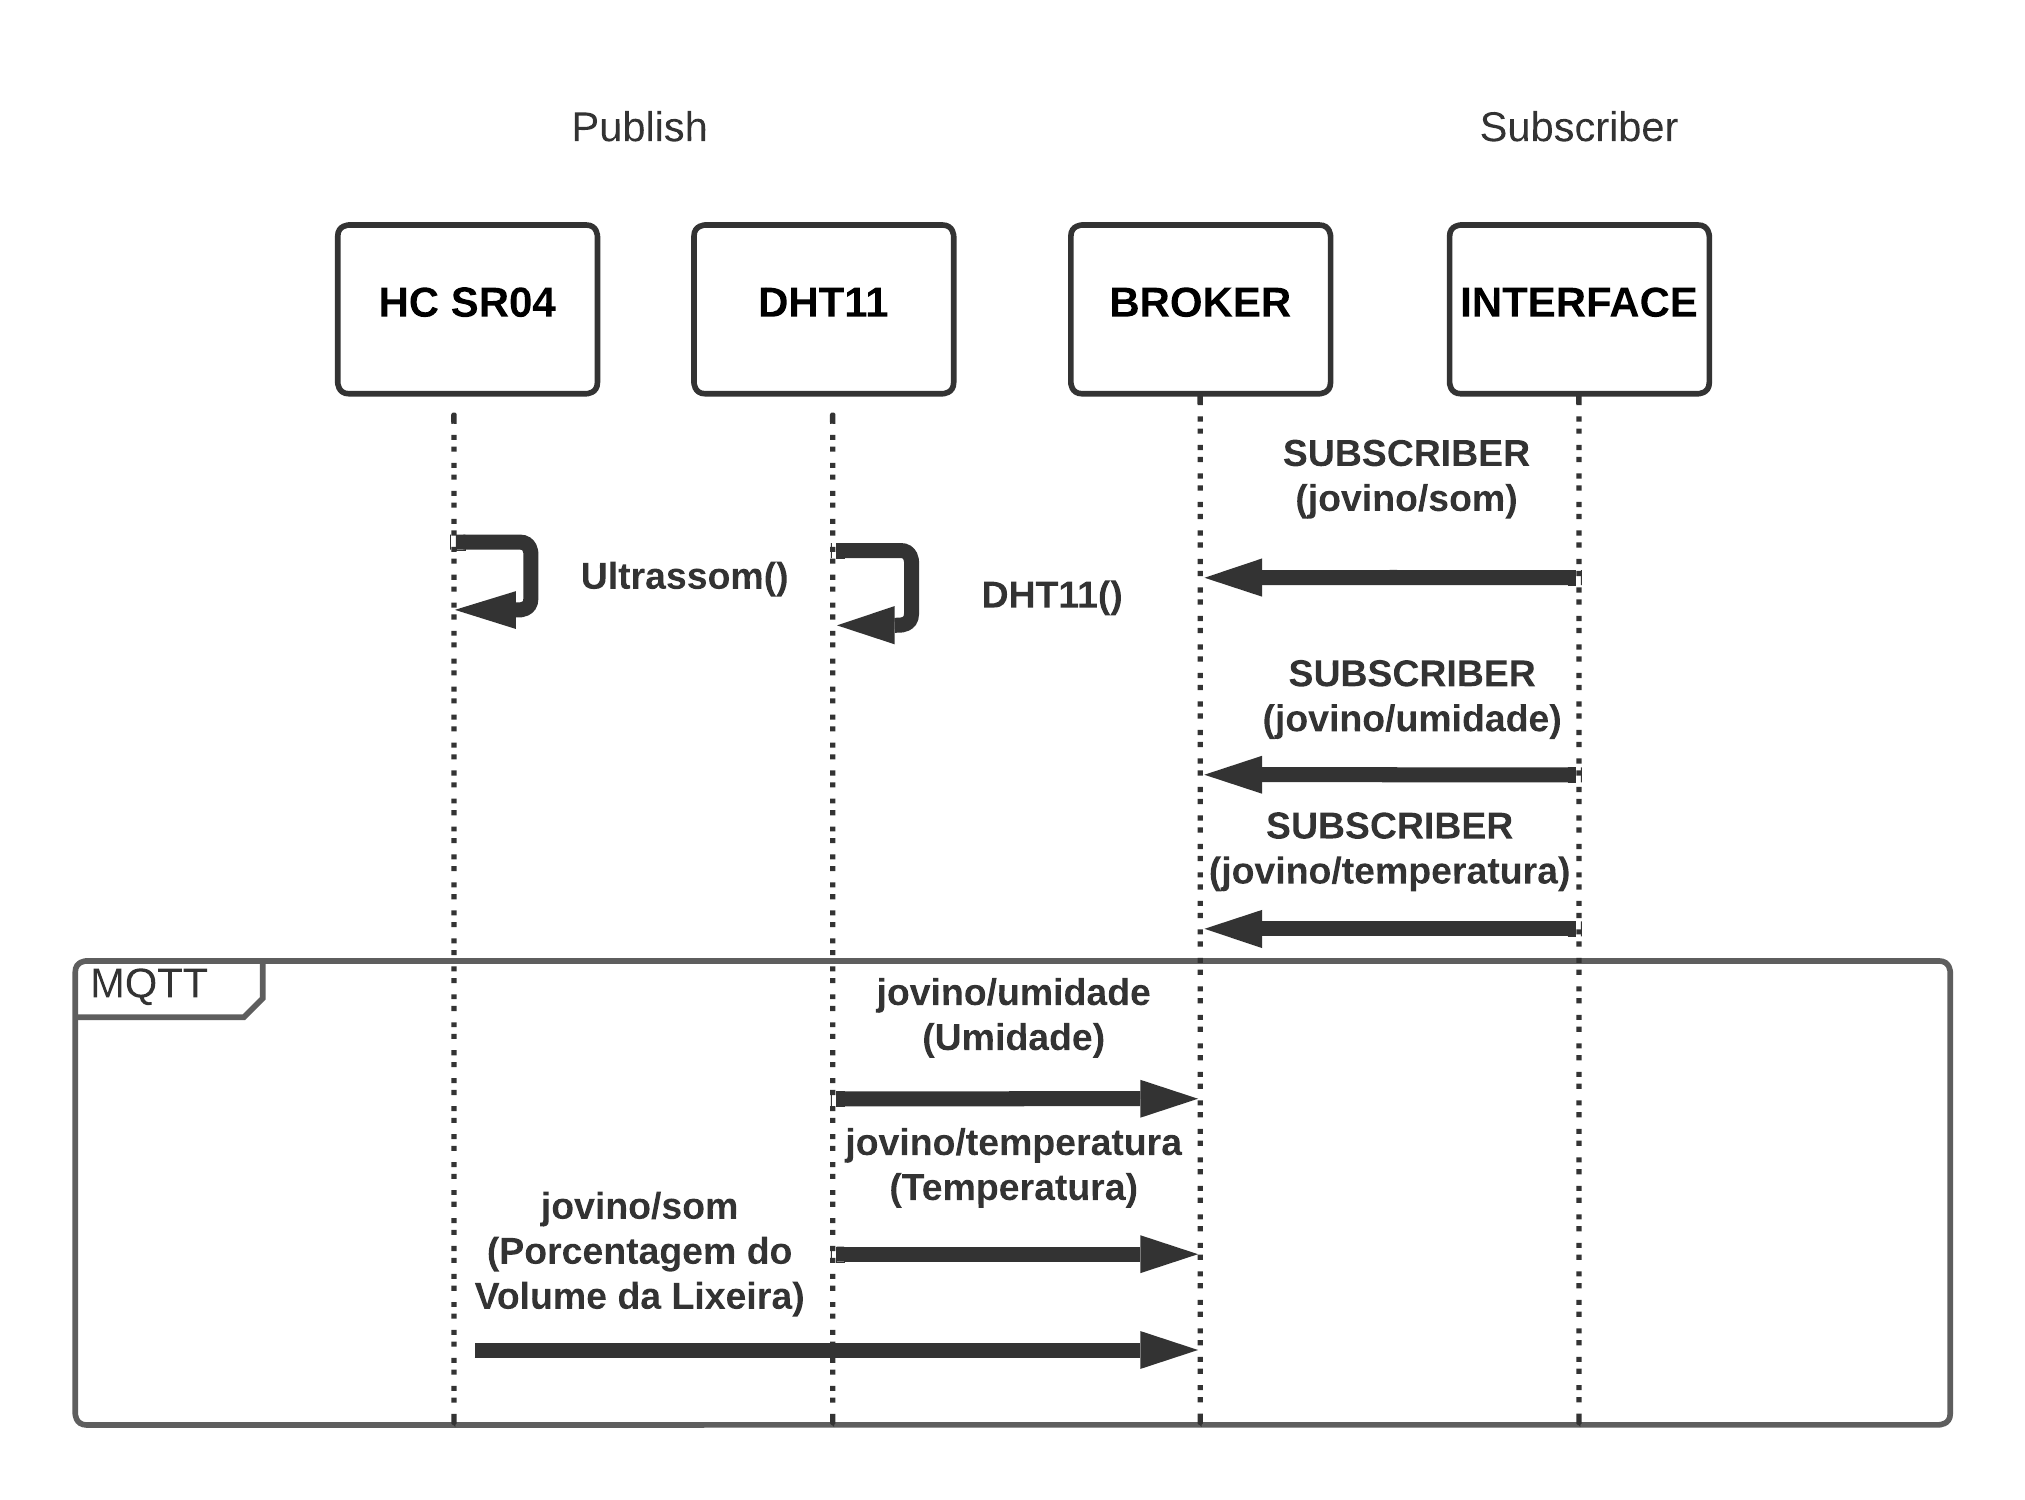
\includegraphics[width=\linewidth]{figures/mqtt.png}
    \caption{Sequência de publicação/assinatura (2024)}
  \end{subfigure}\hfill
  \begin{subfigure}{0.30\textwidth}\centering
    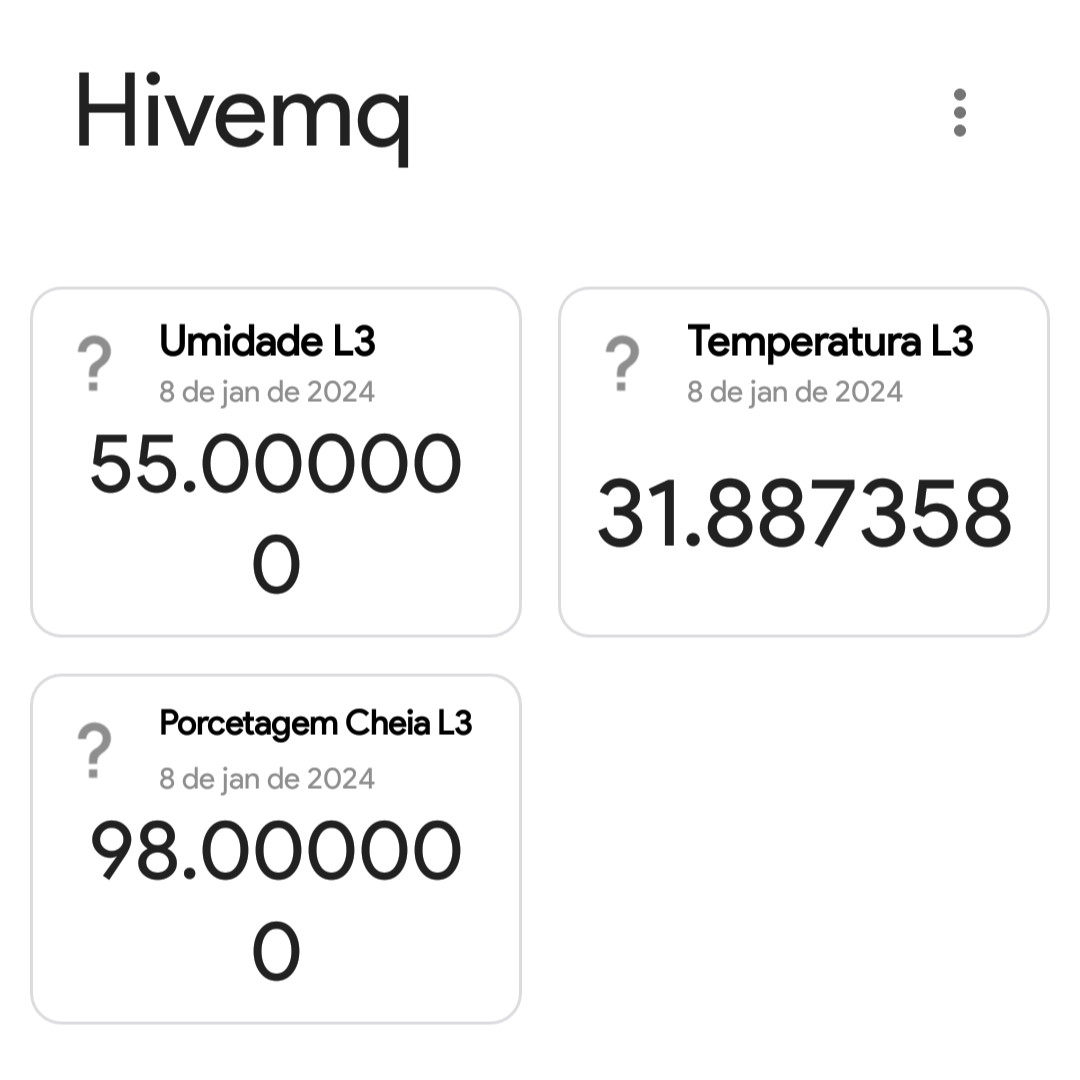
\includegraphics[width=\linewidth]{figures/dashboard.jpg}
    \caption{Aplicativo MQTT Dashboard}
  \end{subfigure}
  \caption{Material do protótipo de 2024, reproduzido do trabalho original.}
  \label{fig:prototipo}
\end{figure}

A auditoria do código original identificou 27 defeitos, cada um verificado no
código e, quando aplicável, na documentação das bibliotecas e nas folhas de
dados. A Tabela~\ref{tab:auditoria} resume os de maior impacto. Dois deles
comprometem diretamente a medida usada no trabalho: a ``porcentagem de volume''
era calculada como $d/T_{\max}\cdot 100$, que \emph{cresce} quando a lixeira
esvazia, e, em caso de eco perdido, a biblioteca de ultrassom usada retornava
51~cm, valor que a fórmula convertia em 102\%. O código também continha
credenciais de Wi-Fi em texto claro, publicadas em repositório público; elas
não são reproduzidas aqui, e recomenda-se trocá-las.

\begin{table}[ht]
\centering
\caption{Principais defeitos do firmware de 2024 e correções (auditoria completa em \texttt{firmware/AUDITORIA.md}).}
\label{tab:auditoria}
\footnotesize
\begin{tabularx}{\textwidth}{@{}>{\raggedright\arraybackslash}p{4.6cm}>{\raggedright\arraybackslash}X@{}}
\toprule
Defeito & Correção no firmware 2.0 \\
\midrule
Percentual proporcional ao espaço vazio, sem limites & ocupação $=100(H-(d-\mathit{off}))/H$, limitada a $[0,100]$ \\
Eco perdido convertido em 51~cm (102\%) & \texttt{pulseIn} com tempo limite; mediana de 5 pulsos com quórum de 3; \texttt{valida=false} \\
Índice de calor publicado como ``temperatura'' & publica a temperatura do ar \\
\texttt{dht.begin()} ausente; LED como entrada & inicialização corrigida \\
Broker público, sem autenticação nem TLS & broker configurável, usuário/senha, TLS opcional \\
Laços bloqueantes de Wi-Fi e MQTT & máquina de estados não bloqueante, recuo exponencial com \emph{jitter} \\
Sem LWT, sem estado, sem sequência & LWT retido, estado \texttt{online}, \texttt{boot} em NVS e \texttt{seq} \\
ECHO (5~V) direto em GPIO de 3,3~V & divisor 1~k$\Omega$/2~k$\Omega$ ($\approx 3{,}33$~V) \\
ECHO no GPIO12 (pino de \emph{strapping} da tensão da flash) & ECHO movido para o GPIO27 \\
Credenciais no código & \texttt{config.h} fora do controle de versão \\
\bottomrule
\end{tabularx}
\end{table}

O firmware 2.0 separa medição, transmissão e rede em módulos e usa um
agendador baseado em \texttt{millis()}, sem \texttt{delay()} no laço principal.
A distância é a mediana de uma rajada de cinco pulsos espaçados em 65~ms (a
folha de dados recomenda ciclo superior a 60~ms \cite{elecfreakssdhcsr04}),
com compensação opcional da velocidade do som pela temperatura do DHT11. A
telemetria é publicada a cada 60~s por padrão, com intervalo ajustável por
comando remoto. Eventos de limiar usam histerese, e um \emph{watchdog} de 30~s
reinicia o dispositivo em caso de travamento.

O firmware foi compilado com o \texttt{arduino-cli} 1.5.1 e o núcleo
\texttt{esp32} 3.3.12 para a placa DOIT ESP32 DevKit~V1, com todos os avisos
habilitados, sem erros nem avisos. A variante padrão ocupa \num{941910} bytes
de flash (71\%) e \num{51284} bytes de RAM estática (15\%). O firmware
\emph{não} foi executado em placa real nem no simulador Wokwi: o protótipo
físico não estava disponível, e a execução automatizada do Wokwi exige uma
credencial que não foi criada. Os arquivos de circuito para o Wokwi estão no
repositório, prontos para uso, mas não constituem resultado deste trabalho.
Assim, o comportamento em tempo de execução do firmware 2.0 permanece não
verificado; o que é verificado em execução é o contrato MQTT, exercitado pelos
dispositivos virtuais.

\subsection{Contrato de mensagens MQTT}

Os tópicos seguem o padrão \texttt{residuos/dispositivos/\{id\}/\{tipo\}}, com
quatro tipos (Tabela~\ref{tab:topicos}). A plataforma assina
\texttt{residuos/dispositivos/+/telemetria}, \texttt{.../+/estado} e
\texttt{.../+/eventos}. A Figura~\ref{fig:mqtt_seq} ilustra a sequência de
conexão, publicação e queda abrupta.

\begin{table}[ht]
\centering
\caption{Tópicos do contrato MQTT (esquema versão 1).}
\label{tab:topicos}
\footnotesize
\begin{tabular}{@{}llccl@{}}
\toprule
Sufixo & Sentido & QoS & Retido & Conteúdo \\
\midrule
\texttt{telemetria} & dispositivo $\to$ plataforma & 0 (ESP32) / 1 (virtual) & não & leituras periódicas \\
\texttt{estado} & dispositivo $\to$ plataforma & 1 & sim & \texttt{online}/\texttt{offline}; LWT \\
\texttt{eventos} & dispositivo $\to$ plataforma & 0/1 & não & limiar, falha de sensor, reinício \\
\texttt{comandos} & plataforma $\to$ dispositivo & 1 & não & intervalo, LED, \emph{ping} \\
\bottomrule
\end{tabular}
\end{table}

\begin{figure}[ht]
  \centering
  \resizebox{\textwidth}{!}{% Sequência MQTT: conexão com LWT, telemetria, falha abrupta
\begin{tikzpicture}[font=\sffamily\tiny, >={Stealth[length=1.7mm]}]
\def\yb{-8.6}
\foreach \x/\n/\c in {0/Dispositivo (ESP32 ou virtual)/orange!12, 6.4/Broker Mosquitto/blue!10, 12.8/Plataforma (ingestão)/green!10}{
  \node[draw, rounded corners=2pt, fill=\c, minimum width=30mm, minimum height=6mm] at (\x,0) {\n};
  \draw[dashed, gray] (\x,-0.3) -- (\x,\yb);}
\draw[->] (12.8,-0.8) -- node[above]{SUBSCRIBE \texttt{.../+/telemetria|estado|eventos} (QoS 1)} (6.4,-0.8);
\draw[->] (0,-1.5) -- node[above, align=center]{CONNECT (id = \texttt{LX-0007}, keepalive 15 s)\\Will: \texttt{.../estado} = offline, QoS 1, retido} (6.4,-1.5);
\draw[->] (0,-2.3) -- node[above]{PUBLISH \texttt{.../estado} = online (retido)} (6.4,-2.3);
\draw[->] (6.4,-2.6) -- (12.8,-2.6);
\foreach \y in {-3.4,-4.1}{
  \draw[->] (0,\y) -- node[above]{PUBLISH \texttt{.../telemetria} \{v, id, boot, seq, ts, leituras\}} (6.4,\y);
  \draw[->] (6.4,\y-0.2) -- (12.8,\y-0.2);}
\node[anchor=west, align=left] at (12.9,-3.9) {valida esquema\\deduplica (id, boot, seq)\\filtro de mediana};
\draw[->] (0,-5.0) -- node[above]{PUBLISH \texttt{.../eventos} \{tipo: limiar\_excedido\}} (6.4,-5.0);
\draw[->] (6.4,-5.2) -- (12.8,-5.2);
\node[red!70!black, font=\sffamily\scriptsize\bfseries] at (0,-6.0) {$\times$ queda sem DISCONNECT};
\draw[->, red!70!black] (6.4,-6.6) -- node[above]{Will: \texttt{.../estado} = offline, motivo = lwt (retido)} (12.8,-6.6);
\draw[->] (0,-7.6) -- node[above]{reconexão com recuo exponencial (1 $\to$ 32 s); estado = online} (6.4,-7.6);
\end{tikzpicture}
}
  \caption{Sequência de mensagens do contrato: conexão com \emph{Last Will}, publicação de estado retido, telemetria, evento e publicação do LWT pelo broker após queda sem DISCONNECT.}
  \label{fig:mqtt_seq}
\end{figure}

Cada telemetria é um objeto JSON com versão do esquema (\texttt{v}),
identificador (\texttt{id}), contador de inicializações persistido em memória
não volátil (\texttt{boot}), número de sequência (\texttt{seq}), instante da
medição (\texttt{ts}), origem do relógio (\texttt{ts\_src}) e uma lista de
leituras, cada uma com tipo, valor, unidade e validade:

\begin{small}
\begin{verbatim}
{"v":1, "id":"LX-0007", "boot":4, "seq":1532, "ts":1731580000, "ts_src":"ntp",
 "leituras":[{"tipo":"distancia","valor":31.2,"unidade":"cm","valida":true},
             {"tipo":"ocupacao","valor":78.8,"unidade":"%","valida":true}]}
\end{verbatim}
\end{small}

O par (\texttt{boot}, \texttt{seq}) identifica unicamente cada mensagem de um
dispositivo, o que permite descartar duplicatas geradas por reentregas com
QoS~1 sem confundi-las com mensagens novas após reinicialização.

\subsection{Ingestão e estado estimado}

A ingestão aplica, nesta ordem: validação de esquema (versão, coerência entre
\texttt{id} e tópico, tipos, unidades e faixa da ocupação); deduplicação por
(\texttt{id}, \texttt{boot}, \texttt{seq}); registro do último contato; descarte
de leituras inválidas para fins de estado; e rejeição, para o estado corrente,
de mensagens com instante anterior ao último estado aplicado ou à última coleta
registrada. A ocupação observada $\hat f_i$ é a mediana das três últimas
leituras válidas do ciclo corrente, o que elimina leituras espúrias isoladas.
Como a mediana introduz um atraso de uma leitura quando há tendência, o
instante associado ao estado é o da leitura mediana, e não o da mais recente;
esse detalhe foi revelado por um teste automatizado.

A taxa de enchimento $\hat r_i$ (fração do volume por hora) é estimada por
mínimos quadrados sobre as leituras das últimas 48~h do ciclo corrente, desde
que haja ao menos 6 leituras cobrindo 12~h; na falta delas, usa-se uma média
móvel exponencial ($\alpha = 0{,}3$) das taxas de ciclos anteriores e, por
último, a mediana das taxas da frota. A projeção para um instante futuro é
$\tilde f_i(t) = \hat f_i + \hat r_i\,(t - t^{\mathrm{obs}}_i)$. Um contêiner
cujo último estado tem mais de 24~h é marcado como \emph{desatualizado}; nesse
caso, as políticas podem usar a estimativa por taxa de longo prazo
(\emph{fallback}) ou manter o último valor observado. Quando um veículo
registra uma coleta, o estado é zerado e um novo ciclo começa.

\subsection{Persistência}

O SQLite armazena todas as mensagens de telemetria recebidas, com o resultado
da ingestão (aplicada, duplicada, fora de ordem ou inválida), o estado de
disponibilidade de cada dispositivo, os eventos, as mensagens rejeitadas, as
rotas planejadas e as coletas executadas. Nos experimentos em lote, os
resultados são gravados em arquivos JSON Lines, uma linha por execução, com a
configuração completa, a semente e as métricas; um manifesto registra o
\emph{commit} do código, as versões das dependências e a plataforma.

\subsection{Simulador}

O simulador é de tempo discreto, com passo de 15~min
(Figura~\ref{fig:simulacao}). Antes da execução, são sorteados, a partir de
fluxos aleatórios independentes derivados da semente, a geometria do cenário,
a matriz de geração de resíduos, os ruídos e falhas dos sensores e as perdas e
atrasos do canal. Como esses sorteios não dependem da política, duas políticas
executadas com a mesma semente enfrentam exatamente as mesmas condições, o que
foi verificado por teste automatizado.

\begin{figure}[ht]
  \centering
  % Laço da simulação em tempo discreto
\begin{tikzpicture}[font=\sffamily\scriptsize, node distance=3.2mm,
  st/.style={draw, rounded corners=2pt, text width=58mm, align=left, inner sep=3pt, fill=#1},
  st/.default=white, arr/.style={-{Stealth[length=1.8mm]}, thick}]
\node[st=gray!10] (init) {\textbf{Inicialização} (semente $s$): malha e posições; matriz de geração $q_{i,t}$; fluxos de ruído, falhas e perdas (números aleatórios comuns a todas as políticas)};
\node[st=red!8, below=of init] (plan) {\textbf{Se $t$ = 06h:} política escolhe contêineres e o OR-Tools gera as rotas do dia a partir do \emph{estado estimado}};
\node[st=orange!10, below=of plan] (gen) {\textbf{Geração:} $f_i \leftarrow f_i + q_{i,t}/V$; excedente acima de $V$ = transbordamento};
\node[st=yellow!15, below=of gen] (truck) {\textbf{Veículos:} avançam até o fim do passo; coletam o volume \emph{verdadeiro}; desvio ao depósito se a carga exceder $Q$; retornam se a jornada não comportar a próxima visita};
\node[st=blue!8, below=of truck] (sense) {\textbf{Sensores:} dispositivos programados medem $d$ (ruído, viés de superfície, falhas) e transmitem pelo canal (perda, atraso, duplicação, interrupções)};
\node[st=green!10, below=of sense] (ing) {\textbf{Ingestão:} mensagens que chegam no passo são validadas, deduplicadas e filtradas; atualiza ocupação e taxa estimadas};
\node[st=purple!8, below=of ing] (met) {\textbf{Métricas} (somente após 7 dias de aquecimento): km, visitas, transbordamento, ocupação na coleta, espera, telemetria, balanço de volume};
\draw[arr] (init) -- (plan);
\foreach \a/\b in {plan/gen, gen/truck, truck/sense, sense/ing, ing/met} \draw[arr] (\a) -- (\b);
\draw[arr] (met.east) -- ++(5mm,0) |- node[pos=0.25, right, align=left] {$t \leftarrow t+1$\\(15 min)} (plan.east);
\end{tikzpicture}

  \caption{Laço da simulação. As decisões usam apenas o estado estimado; o
  estado verdadeiro é usado na geração, na execução das coletas e nas
  métricas.}
  \label{fig:simulacao}
\end{figure}

A separação entre estado verdadeiro e estado estimado é central. As políticas
B, C e D só enxergam o que chegou pela telemetria; o estado verdadeiro é usado
para gerar resíduos, para determinar o volume efetivamente recolhido na
chegada do veículo e para calcular as métricas. A cada execução, o simulador
verifica o balanço de volume na janela avaliada: o volume gerado deve ser igual
à soma do volume coletado, do volume transbordado e da variação do estoque nos
contêineres.

O modo \emph{live} usa as mesmas classes, mas substitui o canal emulado pelo
broker: cada contêiner virtual é um cliente MQTT próprio, com LWT e
reconexão automática (paho-mqtt 2.2, MQTT 3.1.1), e a plataforma é um
assinante com sessão persistente que alimenta a mesma rotina de ingestão.
Nos experimentos em lote, o canal emulado permite processar centenas de
milhares de mensagens por execução; a equivalência entre os dois caminhos é
verificada no experimento E6.

\subsection{Políticas de coleta e roteirização}\label{sec:politicas}

A Figura~\ref{fig:planejamento} resume a decisão diária, tomada às 06h para o
turno das 07h às 15h. As quatro políticas diferem apenas na seleção dos
contêineres e na forma de atribuir prêmios; frota, capacidade, jornada,
velocidade, tempos de atendimento e regra de execução são os mesmos.

\begin{figure}[ht]
  \centering
  \resizebox{0.95\textwidth}{!}{% Fluxo de decisão diária e execução
\begin{tikzpicture}[font=\sffamily\scriptsize,
  b/.style={draw, rounded corners=2pt, align=center, minimum height=9mm, fill=#1},
  b/.default=white, d/.style={draw, diamond, aspect=2.2, align=center, inner sep=1pt, fill=yellow!12},
  arr/.style={-{Stealth[length=1.8mm]}, thick}]
\node[b=green!10, text width=34mm] (est) at (0,0) {Estado estimado\\$\hat f_i$, $\hat r_i$, idade do dado};
\node[d] (stale) at (0,-1.45) {dado\\$>$ 24 h?};
\node[b, text width=30mm] (fb) at (3.6,-1.45) {\emph{fallback}:\\$\hat f_i + \hat r^{\,\mathrm{longo}}_i\,\Delta t$};
\node[d] (pol) at (0,-3.0) {política};
\node[b=red!6, text width=24mm] (A) at (-4.95,-4.6) {\textbf{A}: vencidos no calendário $p_i$ e pendentes};
\node[b=red!6, text width=20mm] (B) at (-1.95,-4.6) {\textbf{B}: $\hat f_i \ge \theta_{hi}$\\(todos obrigatórios)};
\node[b=red!6, text width=24mm] (C) at (1.0,-4.6) {\textbf{C}: obrig. $\hat f_i\ge\theta_{hi}$\\opc. $\hat f_i\ge\theta_{lo}$};
\node[b=red!6, text width=29mm] (D) at (4.45,-4.6) {\textbf{D}: obrig. se $\tilde f_i(t_{\text{meio}})\ge\theta_{hi}$\\ou $\tilde f_i(t_{\text{próx}})\ge\theta_{crit}$};
\node[b=blue!8, text width=96mm] (vrp) at (0,-6.55) {CVRP com prêmios: $\min \sum d_{ij} + \sum_{i\ \text{não visitado}} \pi_i$ \quad (capacidade $Q$, jornada $T_{\max}$, $K$ veículos)\\OR-Tools com descida gulosa (A, B-OR, C, D) ou vizinho mais próximo + 2-opt (B)};
\node[b=yellow!15, text width=96mm] (exe) at (0,-8.25) {Execução com volumes verdadeiros: desvio ao depósito se a carga exceder $Q$;\\visitas que não cabem na jornada ficam não realizadas (A as reprograma para o dia seguinte)};
\draw[arr] (est) -- (stale);
\draw[arr] (stale) -- node[above]{sim} (fb);
\draw[arr] (fb) |- (pol);
\draw[arr] (stale) -- node[left]{não} (pol);
\foreach \x in {A,B,C,D} \draw[arr] (pol) -- (\x.north);
\foreach \x in {A,B,C,D} \draw[arr] (\x.south) -- (\x.south |- vrp.north);
\draw[arr] (vrp) -- (exe);
\end{tikzpicture}
}
  \caption{Decisão diária de coleta e execução das rotas.}
  \label{fig:planejamento}
\end{figure}

\begin{description}
  \item[A -- periódica fixa.] Cada contêiner recebe um período
  $p_i = \min(7, \max(1, \lfloor \gamma V/\mu_i \rfloor))$ dias, em que
  $\mu_i$ é a taxa média de geração de longo prazo e $\gamma = 0{,}8$ é a
  ocupação média desejada na coleta; as fases são distribuídas para equilibrar
  a carga diária. A política usa a taxa média \emph{verdadeira} do simulador,
  o que equivale a um planejador com histórico perfeito. Trata-se de uma
  linha de base deliberadamente exigente: a coleta fixa não é penalizada por
  um mau dimensionamento de frequências. Visitas não realizadas são
  reprogramadas para o dia seguinte.
  \item[B -- limiar.] São obrigatórios os contêineres com $\hat f_i \ge
  \theta_{hi} = 0{,}75$. As rotas são construídas pelo vizinho mais próximo,
  respeitando capacidade e jornada, e melhoradas por 2-opt. A variante B-OR
  usa a mesma seleção com o OR-Tools, para separar o efeito da seleção do
  efeito do roteirizador.
  \item[C -- dinâmica otimizada.] São obrigatórios os contêineres com
  $\hat f_i \ge \theta_{hi}$ e opcionais os com $\theta_{lo} = 0{,}50 \le
  \hat f_i < \theta_{hi}$. O prêmio de um opcional é $\pi_i = \lambda\,\hat
  f_i V$, com $\lambda = 1$~m por litro: o contêiner entra na rota se o desvio
  necessário for menor que o prêmio.
  \item[D -- preditiva.] Como C, mas com ocupações projetadas pela taxa
  estimada. É obrigatório o contêiner cuja projeção para o meio do turno é
  $\ge \theta_{hi}$ ou cuja projeção para o fim do turno seguinte é $\ge
  \theta_{crit} = 0{,}95$, isto é, que provavelmente transbordaria antes da
  próxima oportunidade de coleta.
\end{description}

O problema diário é um CVRP com prêmios. Sejam $S$ o conjunto de contêineres
selecionados, $K$ o número de veículos, $Q$ a capacidade por viagem, $q_i$ o
volume estimado, $d_{ij}$ a distância na malha (assimétrica, por causa das vias
de sentido único), $t_{ij}$ o tempo de viagem, $s$ o tempo de atendimento e
$T_{\max}$ a jornada. O resolvedor busca rotas $R_1,\dots,R_K$ que minimizem
\begin{equation}
  \sum_{k=1}^{K}\sum_{(i,j)\in R_k} d_{ij} \;+\; \sum_{i\in S\setminus \cup_k R_k} \pi_i
  \label{eq:objetivo}
\end{equation}
sujeitas a $\sum_{i\in R_k} q_i \le Q$ e $\sum_{(i,j)\in R_k}(t_{ij}+s) \le
T_{\max}$ para todo $k$. Contêineres obrigatórios recebem $\pi_i = 10^8$,
valor superior a qualquer distância possível, de modo que só são omitidos
quando não há solução viável que os inclua. O OR-Tools 9.15 é configurado com
solução inicial pelo arco mais barato e busca local por descida gulosa até um
ótimo local. Essa configuração é determinística: a mesma entrada produz sempre
a mesma rota, independentemente da velocidade da máquina. O efeito de
substituí-la pela busca local guiada, interrompida por tempo, é medido no
experimento E5.

Na execução, o veículo chega a cada contêiner e recolhe o volume verdadeiro
naquele instante. Se a carga excederia $Q$, ele vai ao depósito, descarrega e
retorna \cite{dror1989vehicle}; se a jornada não comporta a próxima visita e o
retorno, ele encerra a rota, e as visitas restantes são registradas como não
realizadas.

\subsection{Painel operacional}\label{sec:painel}

O painel web foi construído com FastAPI no servidor e HTML, CSS e JavaScript
sem bibliotecas externas no navegador, para funcionar sem acesso à internet.
Ele lê exclusivamente dados produzidos pela aplicação: o estado escrito pelo
modo \emph{live} a cada passo, o banco SQLite alimentado pela ingestão MQTT,
um traço gravado de simulação e o resumo dos experimentos. Há três visões:

\begin{itemize}
  \item \textbf{Operação ao vivo} (Figura~\ref{fig:painel}a): mapa da malha
  viária com os contêineres coloridos pela ocupação estimada, contêineres sem
  dado recente em contorno, dispositivos \emph{offline} marcados, depósito,
  veículos e rotas do dia desenhadas pelas ruas; indicadores de distância,
  coletas, transbordamento, dispositivos \emph{online} e mensagens
  (recebidas, duplicadas e rejeitadas); filtros por estado; histórico de
  telemetria de cada contêiner, consultado no SQLite; e lista de eventos
  MQTT. Um seletor alterna entre o estado estimado pela plataforma e o estado
  verdadeiro do simulador, o que permite observar a diferença entre o que o
  operador vê e o que de fato ocorre.
  \item \textbf{\emph{Replay} A $\times$ D} (Figura~\ref{fig:painel}b):
  reprodução sincronizada de duas execuções com a mesma semente, com controle
  de tempo e velocidade.
  \item \textbf{Resultados}: tabela do experimento E1 e fronteira do E2, lidas
  do resumo gerado pela análise.
\end{itemize}

\begin{figure}[ht]
  \centering
  \begin{subfigure}{\textwidth}\centering
    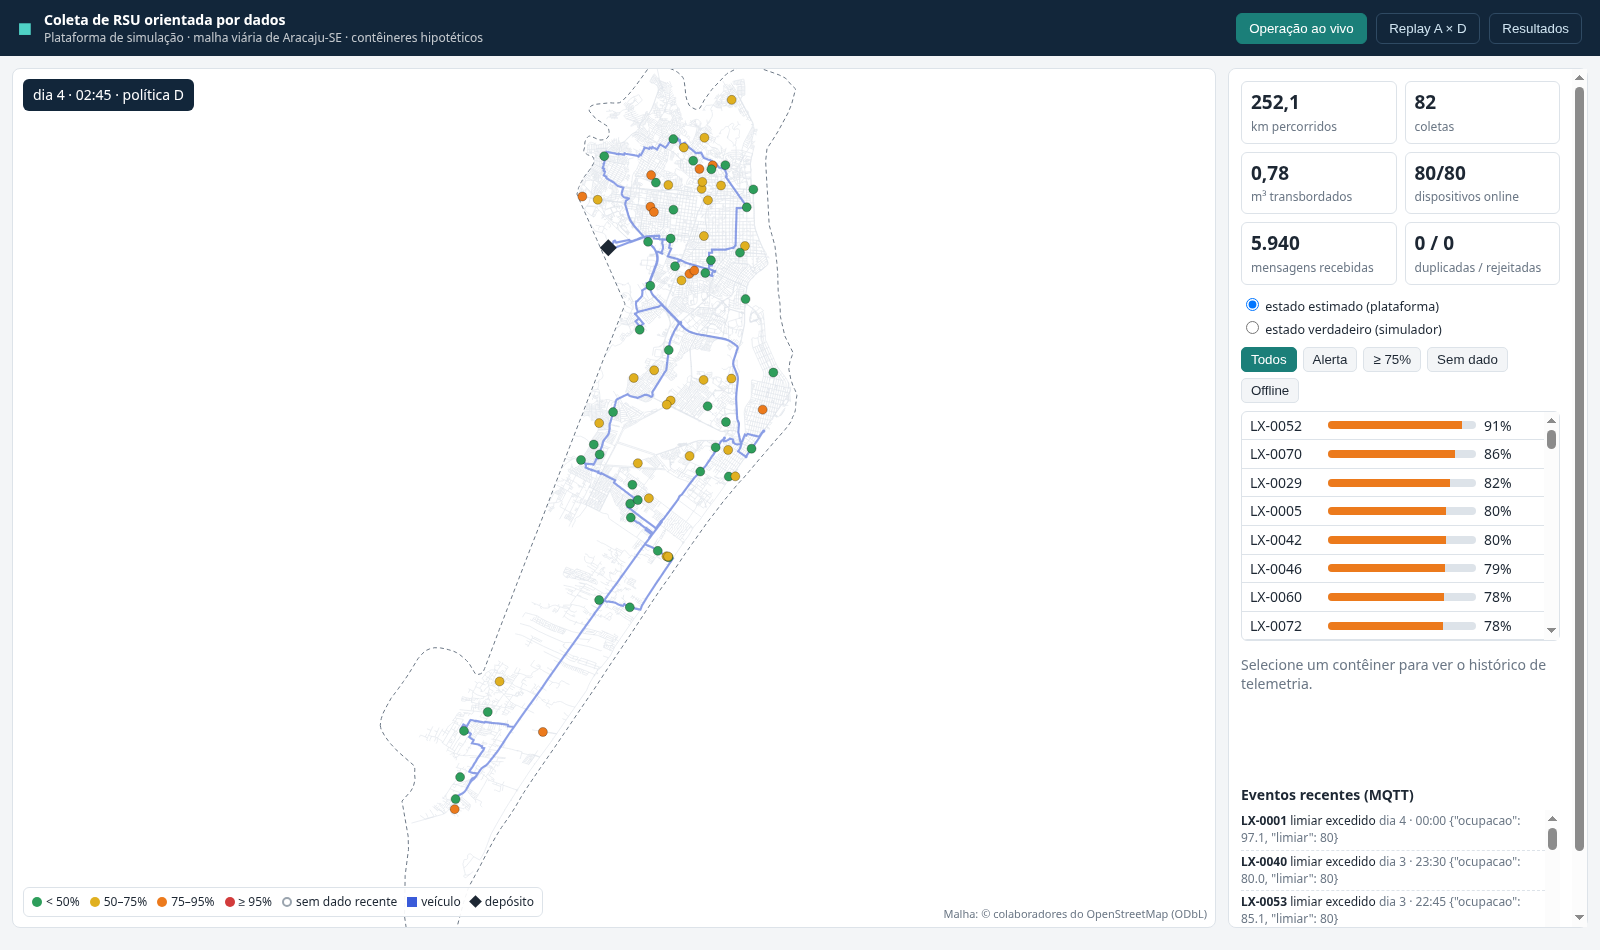
\includegraphics[width=0.93\textwidth]{figures/painel_ao_vivo.png}
    \caption{Operação ao vivo: telemetria recebida pelo broker, rotas do dia e histórico de um contêiner.}
  \end{subfigure}\\[4pt]
  \begin{subfigure}{\textwidth}\centering
    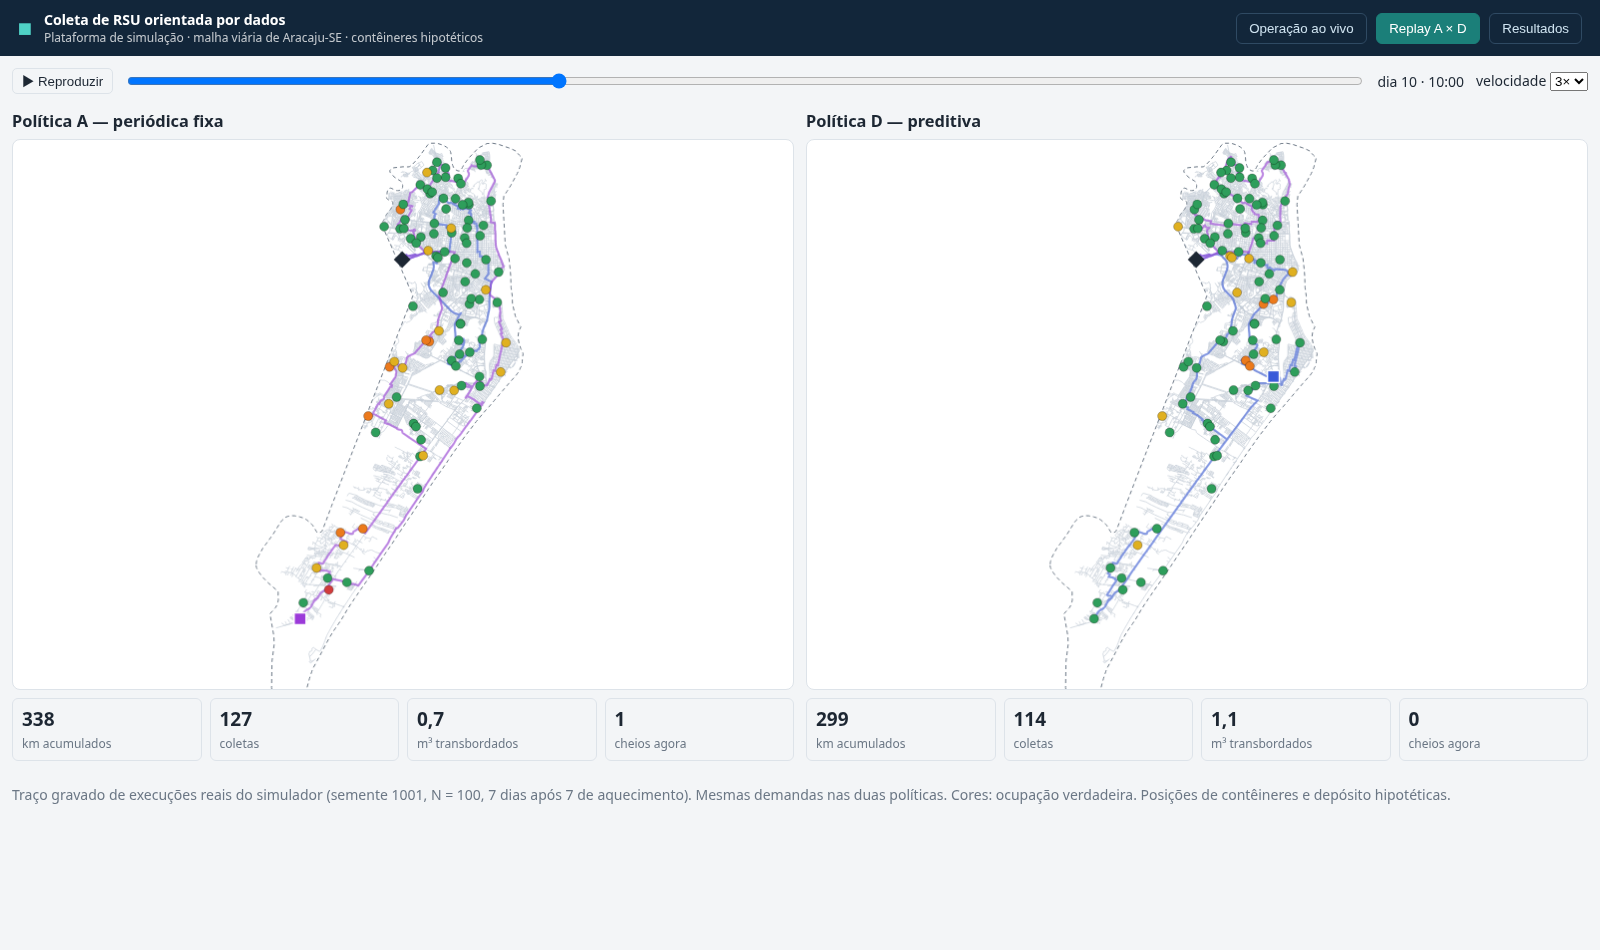
\includegraphics[width=0.93\textwidth]{figures/painel_replay.png}
    \caption{Replay sincronizado das políticas A e D (semente 1001, $N = 100$).}
  \end{subfigure}
  \caption{Capturas do painel operacional, obtidas com a aplicação em execução (navegador em modo \emph{headless}).}
  \label{fig:painel}
\end{figure}


\subsection{Verificação do software}

O pacote tem \NTestes{} testes automatizados (pytest), que cobrem: a fórmula de
ocupação e seus limites físicos; leituras inválidas; o viés de superfície do
modelo de sensor, comparado ao valor teórico $\sigma\sqrt{2/\pi}$; a fração de
indisponibilidade do processo de falhas, comparada a
$\mathrm{MTTR}/(\mathrm{MTBF}+\mathrm{MTTR})$; a média de longo prazo da
geração; o determinismo por semente; a validação do esquema de mensagens; a
deduplicação, a ordenação e o filtro de mediana; a estimativa de taxa em uma
série linear; o roteirizador em instâncias pequenas, comparado à enumeração
exata; o respeito à capacidade e à jornada; o balanço de volume para as quatro
políticas; e o uso de números aleatórios comuns entre políticas.
